\section{Saving System State: Snapshots}

\label{sec:snap}
This section discusses saving state. This is useful for fault-tolerance and system migrations.

\begin{Def}[Snapshot]
    
    \label{def:snapshot}
    A \textbf{snapshot} is a consistent global state of a distributed system at a specific point in time. 
\end{Def}

\begin{Def}[Consistent vs. Inconsistent Snapshots]

    \label{def:consistency}
    To evaluate a snapshot's consistency, we compare events in the system \textbf{pre-snapshot} (events before the snapshot) 
    and \textbf{post-snapshot} (events after the snapshot). The snapshot itself is instantaneous, like a photograph. 
    Given an event ordering $r$:
    
    \begin{itemize}
        \item \textbf{Consistent Snapshots}: Respect causal dependencies. Let there be events $e_1$ and $e_2$; If $e_1 \rightarrow_r e_2$, then $e_1$ must be included in the snapshot if $e_2$ is present.
        \item \textbf{Inconsistent Snapshots}: Violate causal dependencies. If $e_2$ is included without 
        the causally preceding event $e_1$, then the snapshot is inconsistent.
    \end{itemize}
\end{Def}

\vspace{-1em}
\begin{figure}[h]
    \centering
    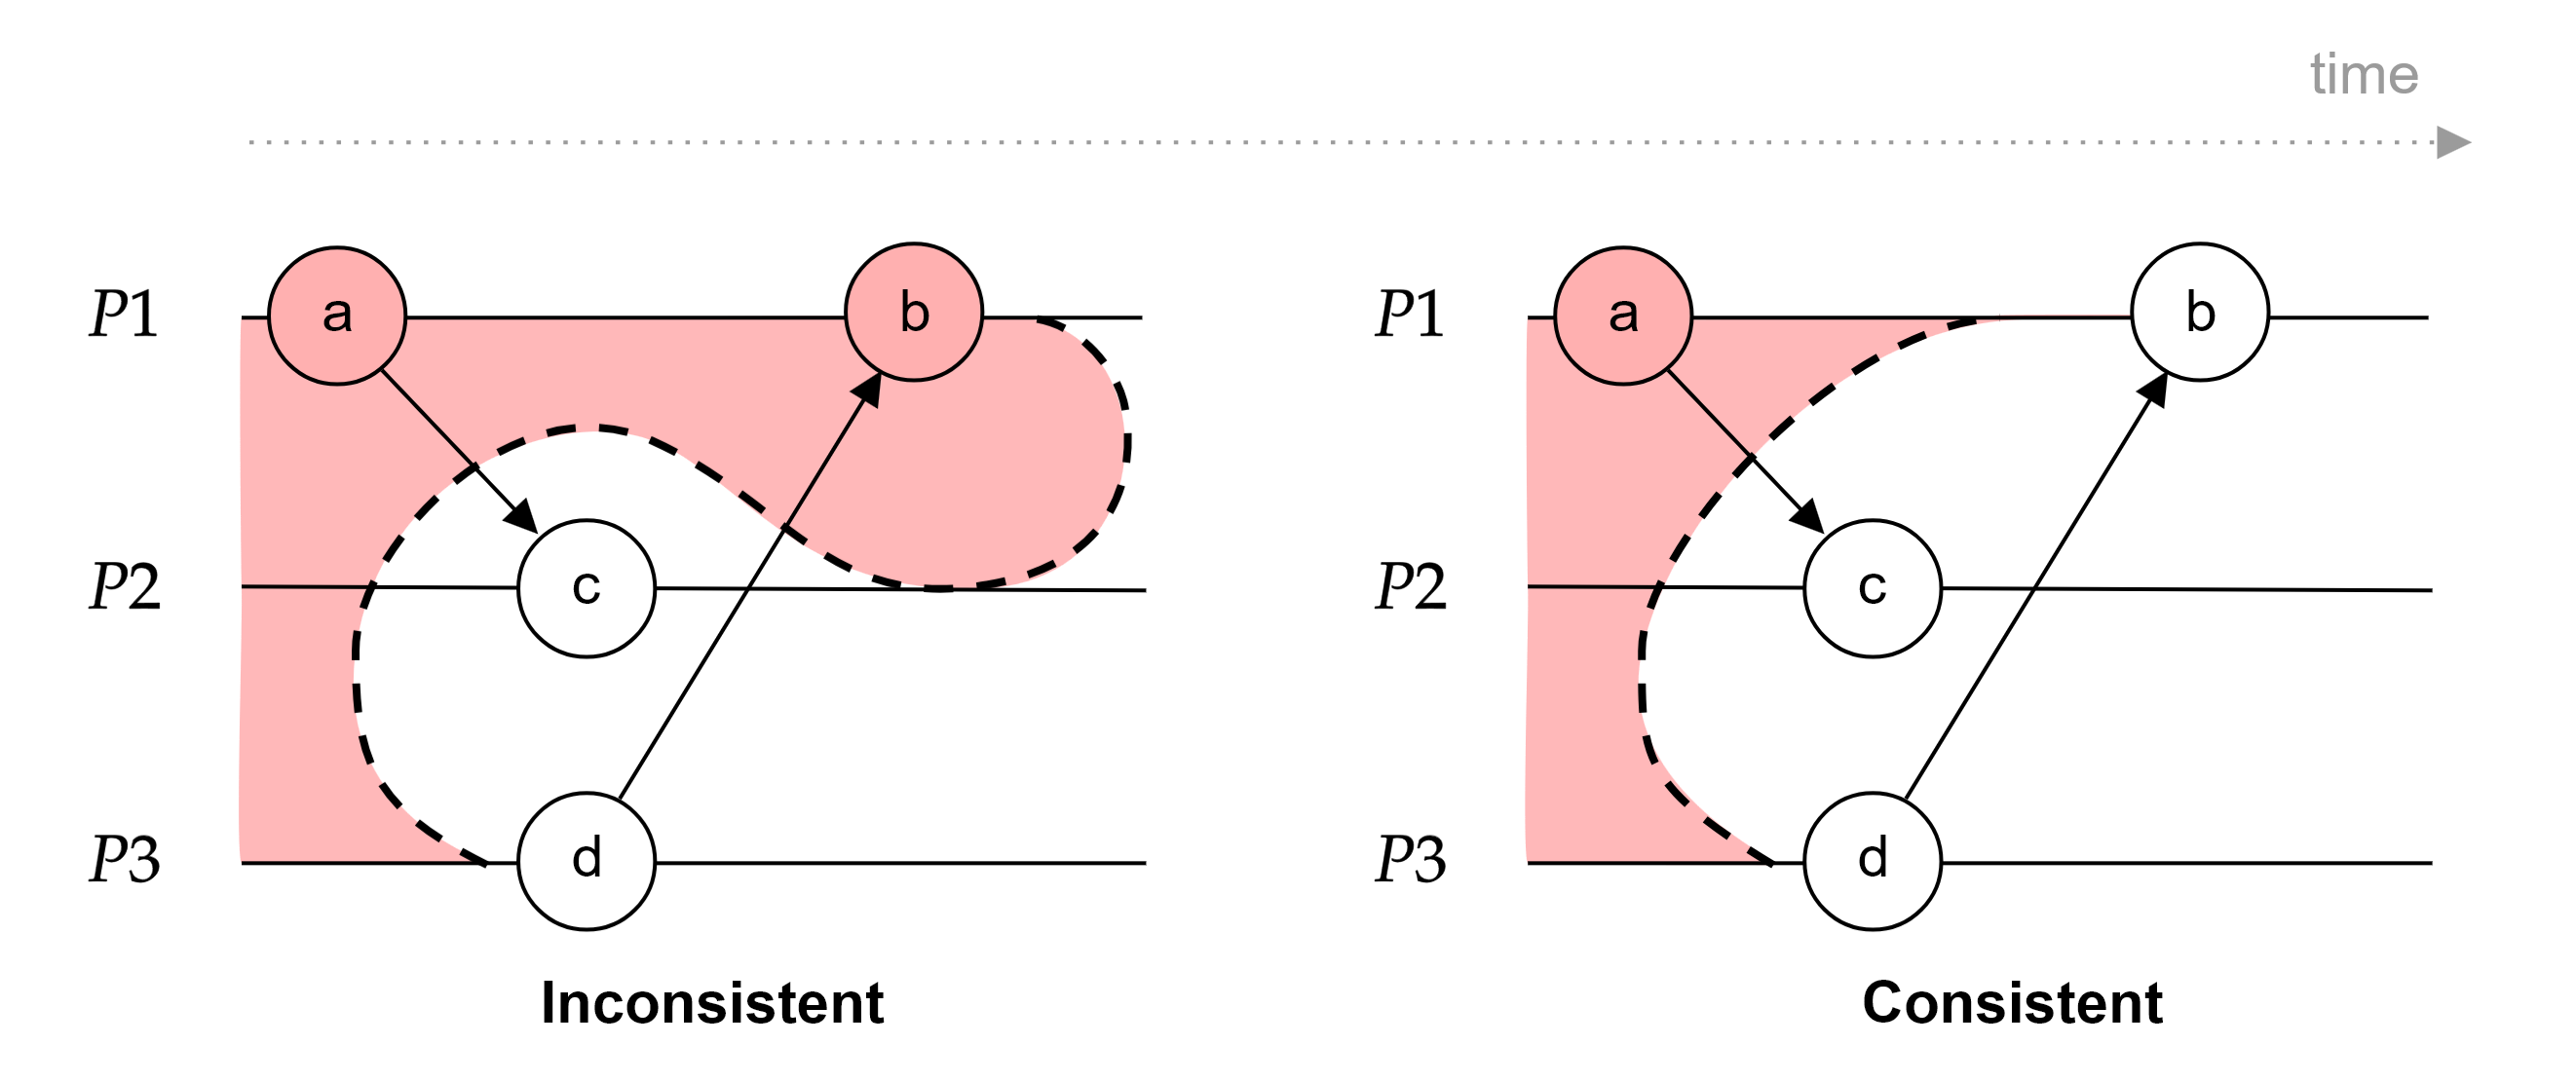
\includegraphics[width=.9\textwidth]{Sections/snap/snap.png}
    \caption{Inconsistent vs. Consistent Snapshots (pre-snapshot highlighted in red)}
\end{figure}

\noindent 
Here, in the inconsistent snapshot, $b$ is included without $d$, its causally preceding event. In the consistent snapshot, only $a$ is 
included. In this snapshot $c$ and $d$ could be added without violating causality.

\newpage 

\noindent 
There are many snapshot protocols, but we will focus on the \textbf{Chandy-Lamport Algorithm}.
\begin{Def}[Chandy-Lamport Algorithm]

    The \textbf{Chandy-Lamport Algorithm} is a snapshot algorithm that is used in distributed systems for
    recording a consistent global state of an asynchronous system. In this protocol:
    \begin{itemize}
        \item The snapshot procedure does not disrupt other processes.
        \item Each process records its local state.
        \item Any process can initiate the snapshot.
    \end{itemize}
    \noindent
    This model requires: 
    \begin{itemize}
        \item \textbf{No Failures}: No failures during the snapshot.
        \item \textbf{First in, First out Channels (FIFO)}: no lost or duplicated messages.
        \item \textbf{Strongly Connected Network}: All processes can reach every other process.
        \item \textbf{Single Initiator}: Only one process can initiate the snapshot.
    \end{itemize}
    
    \noindent 
    The initiator then:
    \begin{itemize}
        \item Sends a \textbf{Marker} message to all outgoing channels.
        \item Records local and incoming channel data.
    \end{itemize}
    Recipients of the marker message:
    \begin{itemize}
        \item Designates the channel which the marker arrived as \textbf{empty}.
        \item Records their local state and all other incoming channels \underline{except the empty one}.
        \item Sends the marker to all outgoing channels.
    \end{itemize}
    \noindent
    \textbf{Completion}: When all processes have received and sent a marker, the snapshot is complete. This 
    means every processes incoming channel is empty, hence the conclusion of the snapshot.

    \noindent
    \rule{\textwidth}{0.4pt}\\

    \noindent
    \textbf{Important Notes}:
    \begin{itemize}
        \item Subsequent markers received are ignored, \textbf{only the first} marker received is acted upon.
        \item Without the FIFO property, restarting the system may not be possible, as it relies on the order of messages to 
        reproduce state.
    \end{itemize}
\end{Def}

\newpage 

\noindent 
Observe the following illustration of the Chandy-Lamport Algorithm given processes $p_1, p_2, p_3$:
\begin{figure}[h] 
    \centering
    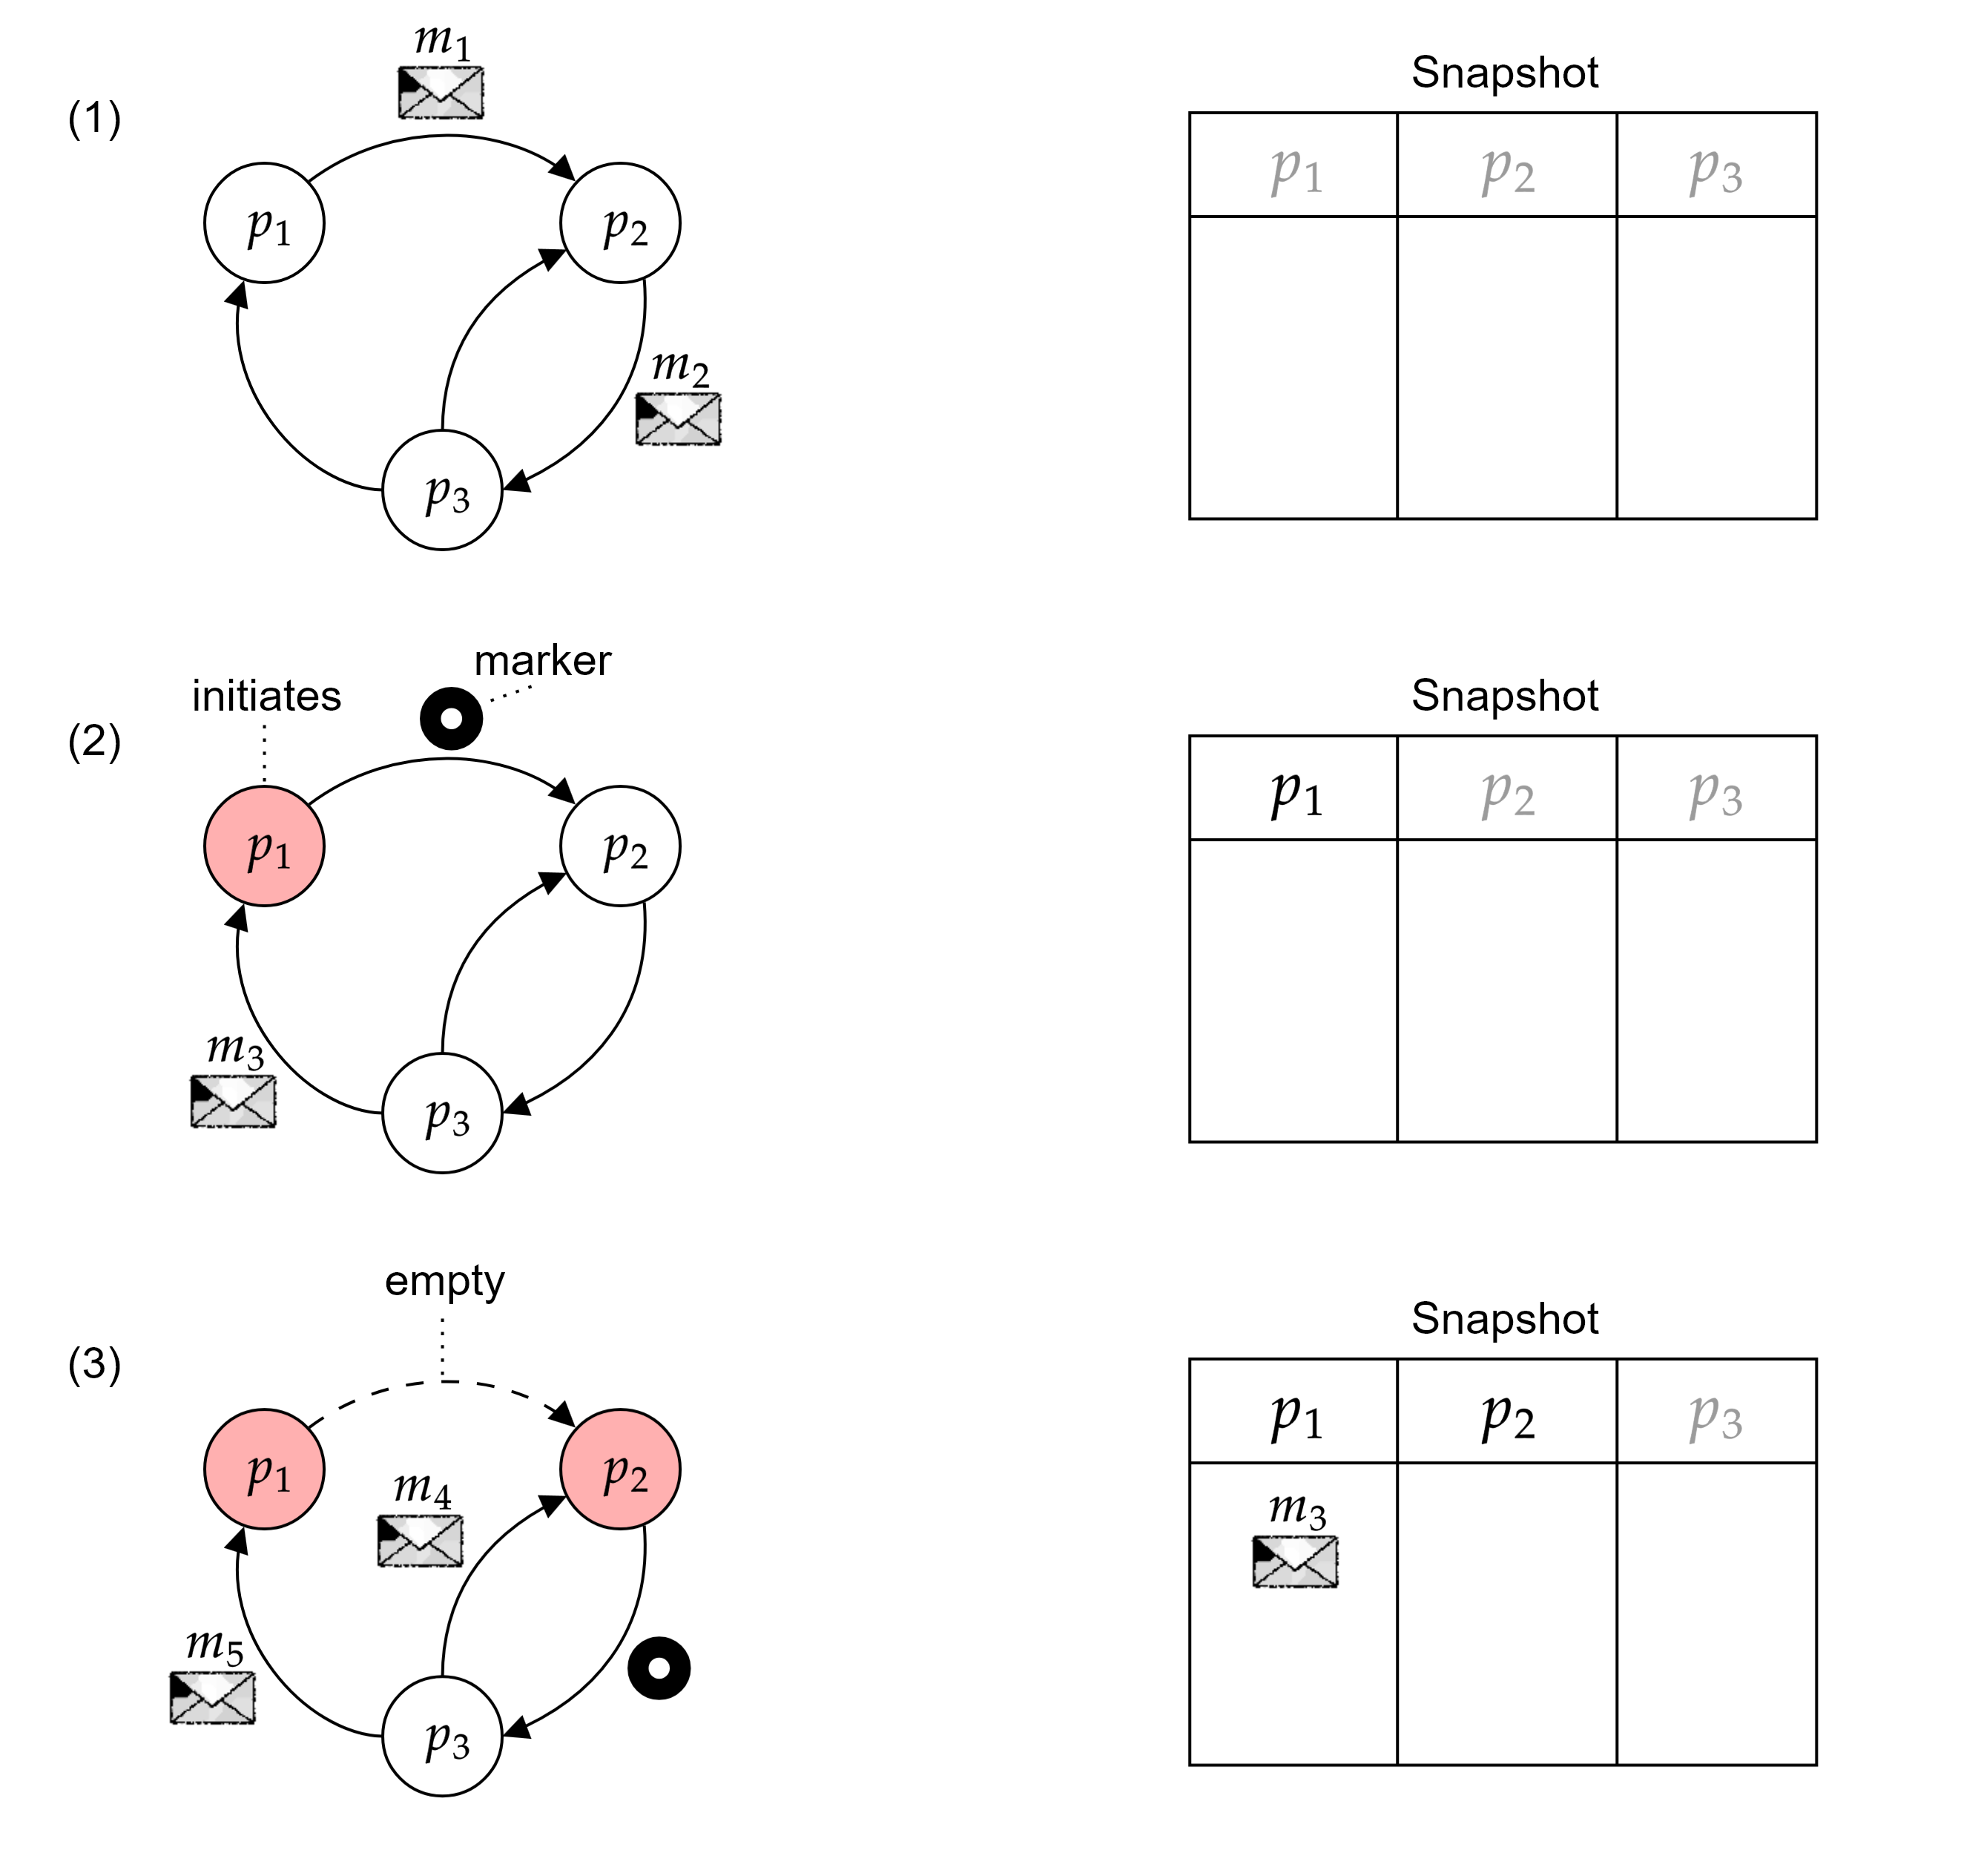
\includegraphics[width=1\textwidth]{Sections/snap/snap_exe.png}
\end{figure}

\noindent
Examining these first three steps: (1) The system before the snapshot. (2) $p_1$ initiates the snapshot sending a marker to $p_2$ and recording its local and incoming channel's state. 
(3) $p_2$ receives the marker, designating the incoming channel from $p_1$ as empty, sends the marker on outgoing channels, and begins recording. We also see, $p_1$ has recorded an incoming message $m_3$ from (2).\\

\noindent
We continue on the next page.

\newpage 

\noindent
We continue the snapshot process with the following steps:
\begin{figure}[h] 
    \centering
    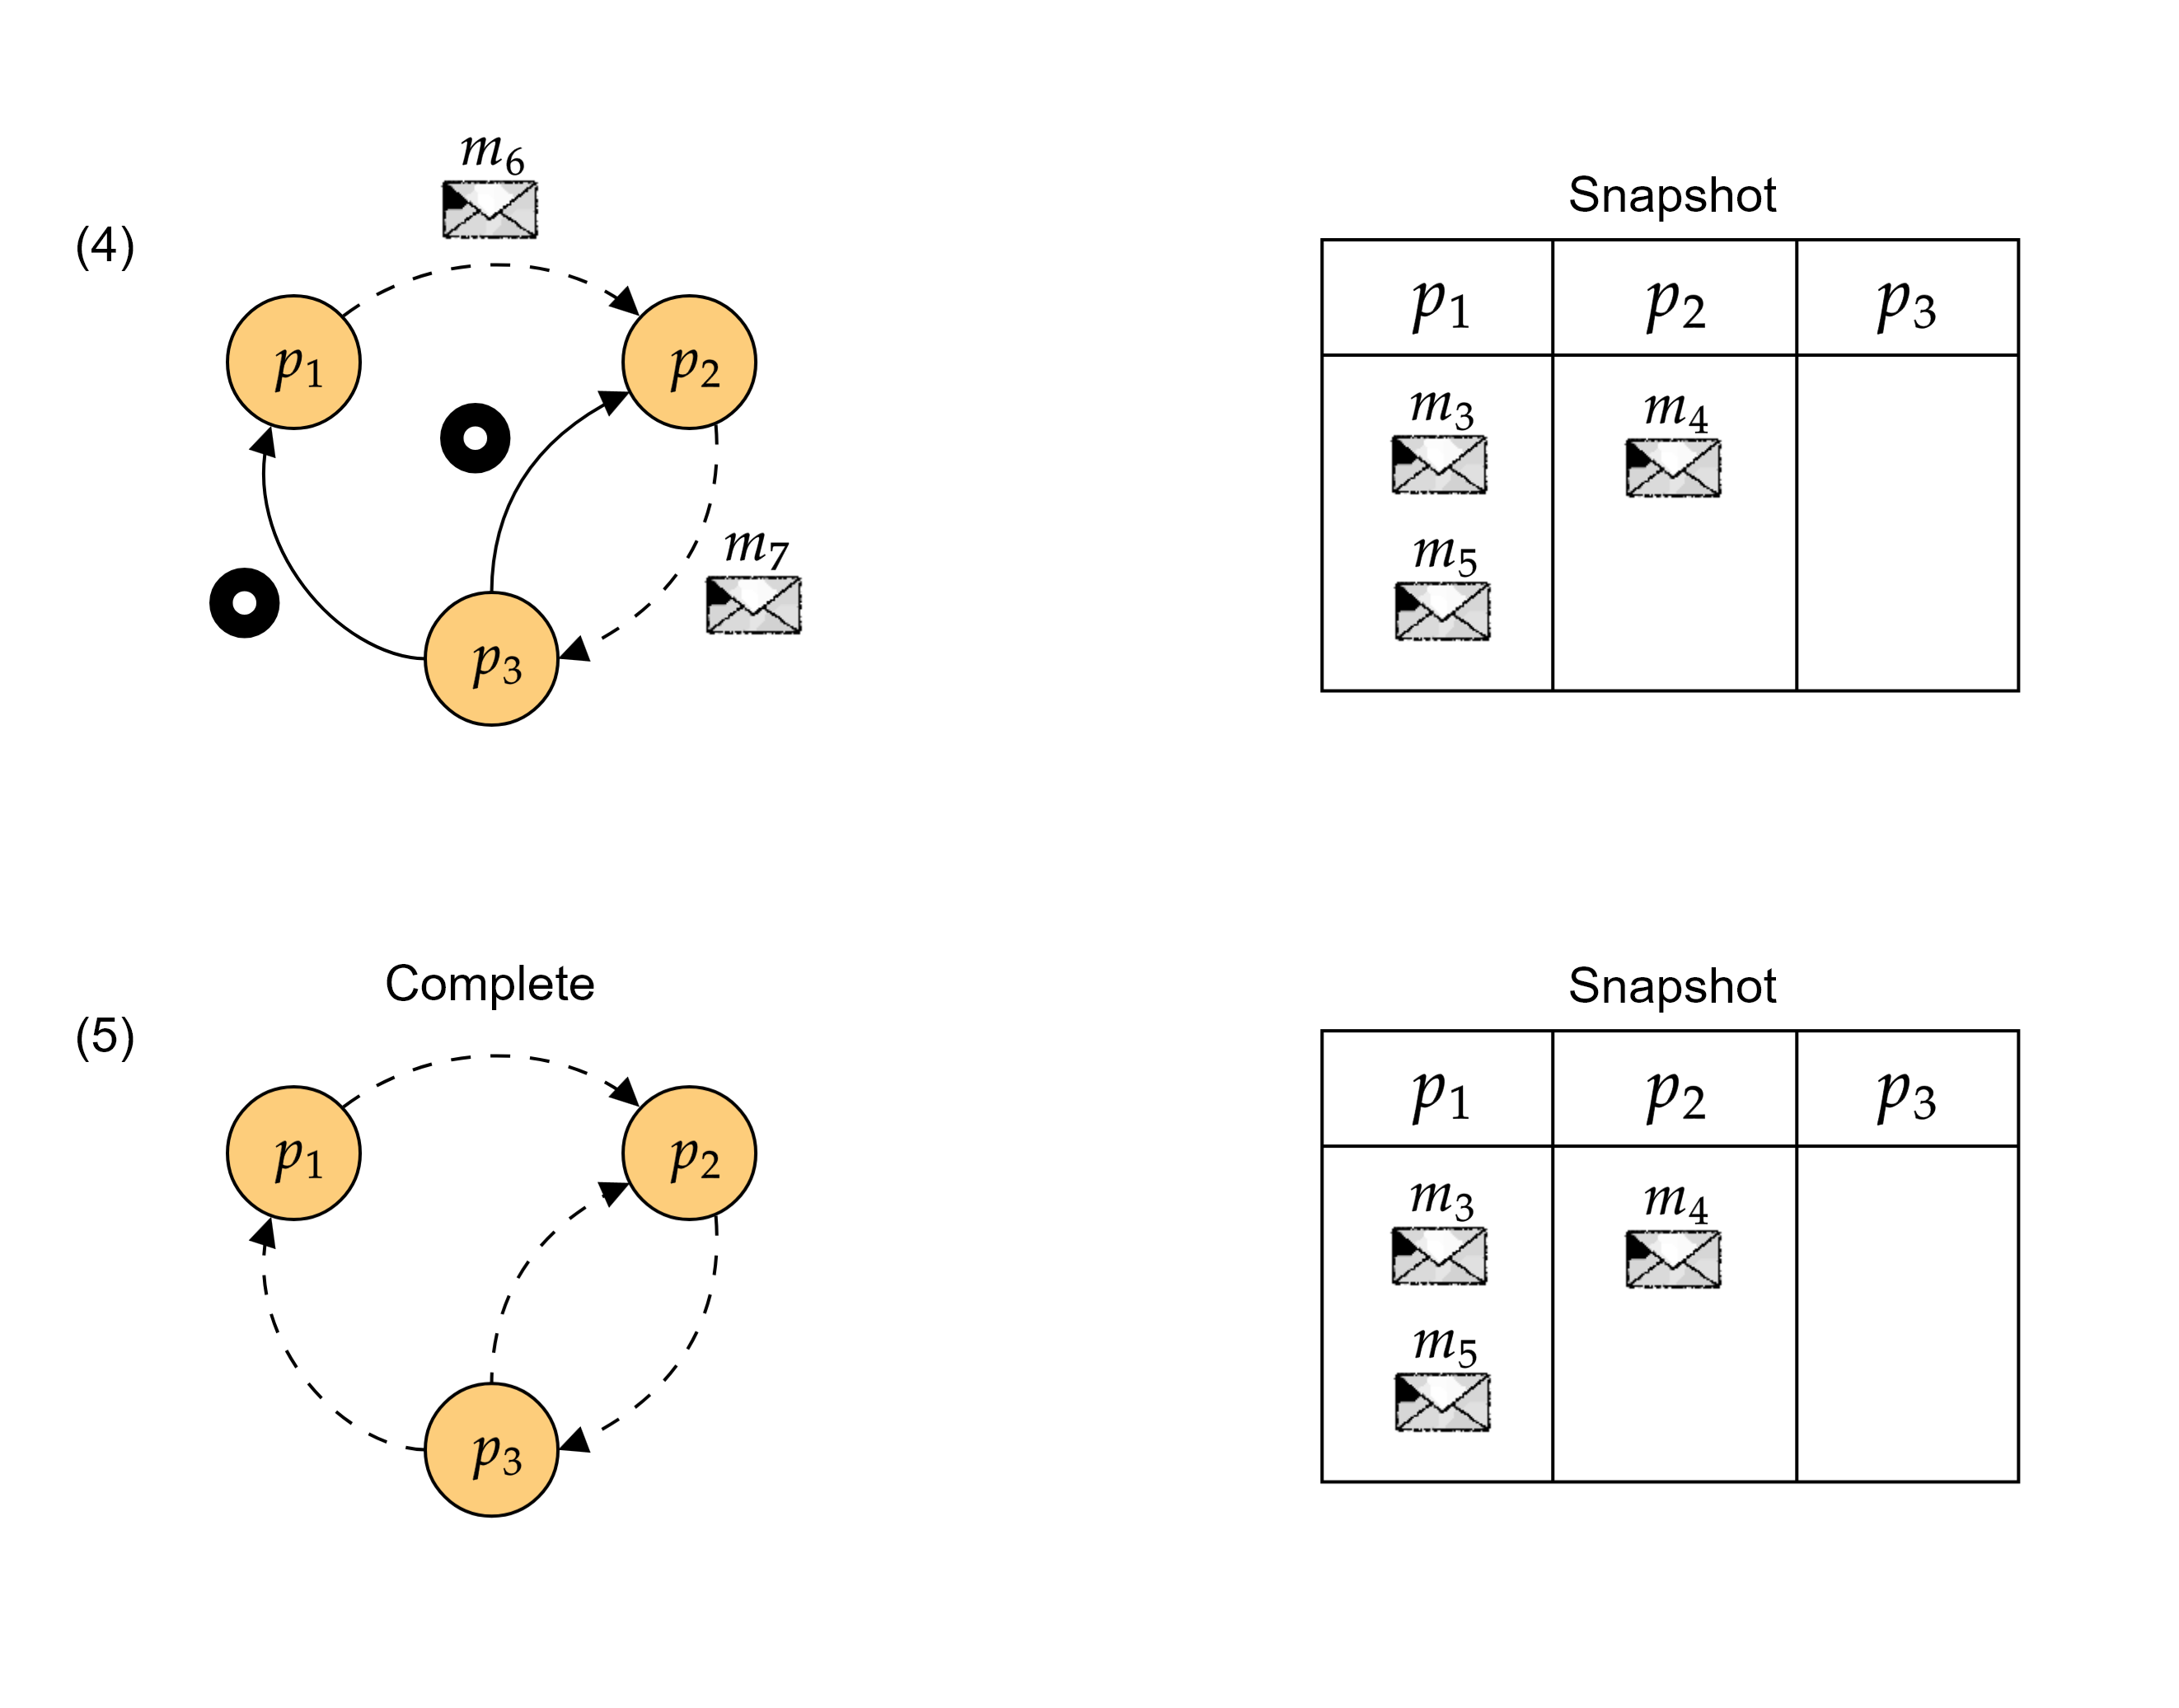
\includegraphics[width=1\textwidth]{Sections/snap/snap_exe_2.png}
\end{figure}

\noindent
(4) $p_3$ received the marker from $p_2$, and designates that incoming channel as empty. It begins recording state, sending out the marker to $p_1$ and $p_2$.
Take notice that messages $m_4$ and $m_5$ have been recorded from (3).
(5) All channels are now empty, concluding the snapshot. Take note that $m_6$ and $m_7$ were not recorded as they were sent on empty channels.\\

\begin{theo}[Replay of a Snapshot]

    When replaying a snapshot captured using the Chandy-Lamport protocol, 
    messages in transit (i.e., sent by a task whose state was recorded, but not yet received by others) 
    \textbf{must also be replayed}. \\

    \noindent
    In particular, if task $A$ sends a message to task $B$, and only $A$ is included in the snapshot,
    then the message is considered in transit and must be delivered to $B$ upon replay.
\end{theo}


\newpage 

\noindent
Consider the following illustrations and think about how many messages may be replayed:

\begin{figure}[h]
    \centering
    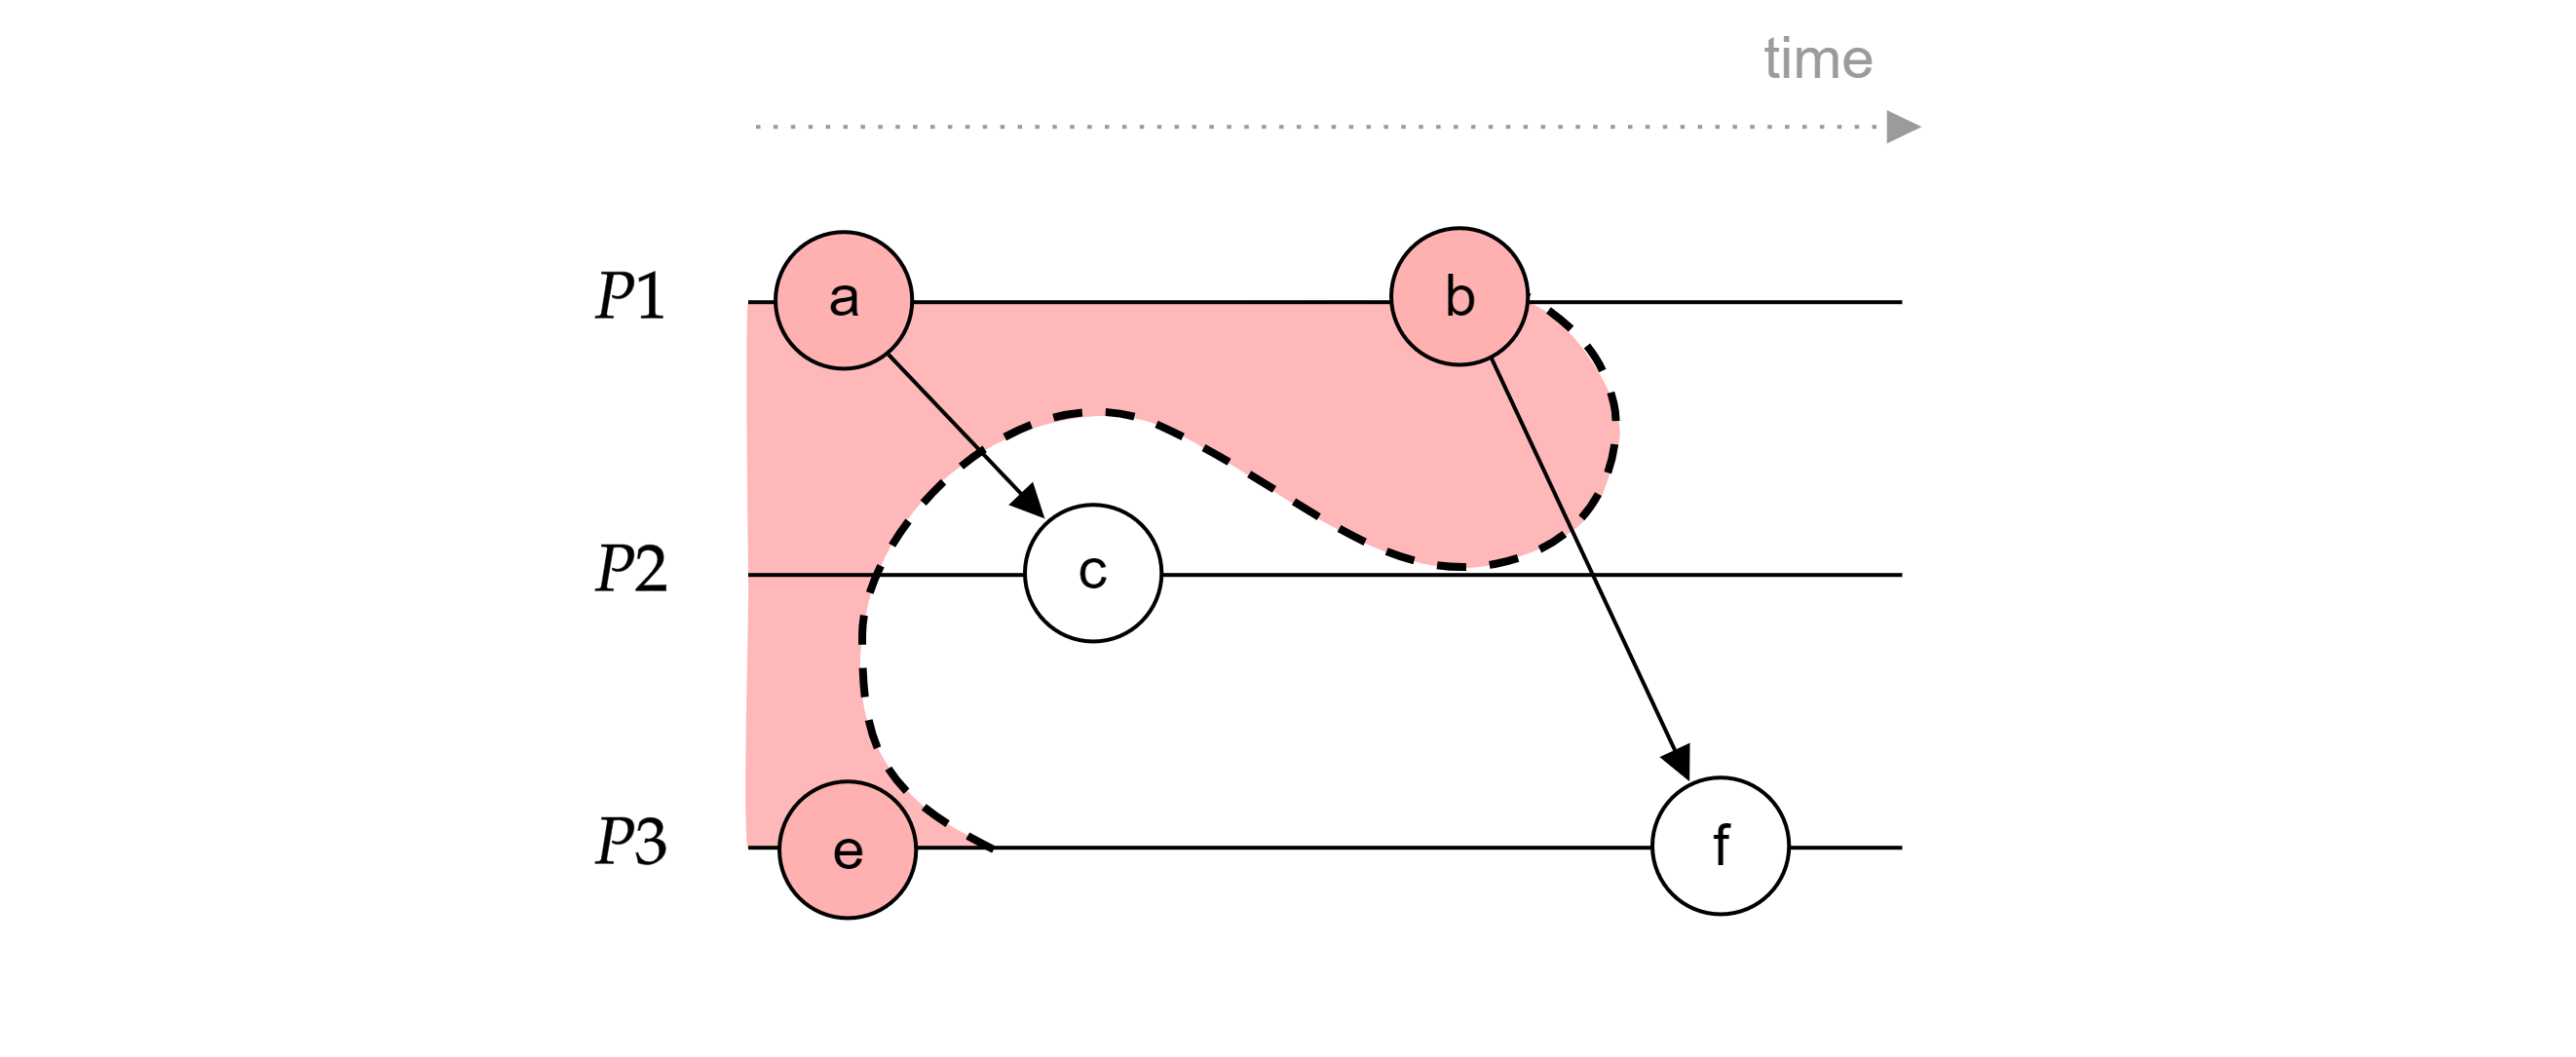
\includegraphics[width=1\textwidth]{Sections/snap/snap_2.png}
    \caption{tasks $a,b$ and $e$ are recorded in the snapshot. Both $a$ and $b$ send messages from which aren't recorded in the snapshot. After 
    reloading the snapshot, $a$ and $b$'s messages \textbf{must be replayed}.}
\end{figure}
